\documentclass[12pt]{beamer}

\usetheme{Air}
\usepackage[czech]{babel}
\usepackage{thumbpdf}
\usepackage{wasysym}
\usepackage{ucs}
\usepackage[utf8]{inputenc}
\usepackage{verbatim}

\pdfinfo
{
  /Title       (Web Services)
  /Creator     (TeX)
  /Author      (Matěj Laitl, Matěj Novotný)
}


\title{Web Services}
\subtitle{Aby byly strojově čitelné zprávy čitelné i pro vás}
\author{Matěj Laitl, Matěj Novotný}
\date{\today}

\begin{document}

\frame{\titlepage}

\section*{}
\begin{frame}
  \frametitle{Co si dnes povíme}
  \tableofcontents[section=1,hidesubsections]
\end{frame}

\AtBeginSection[]
{
  \frame<handout:0>
  {
    \frametitle{Přehled}
    \tableofcontents[currentsection,hideallsubsections]
  }
}

\AtBeginSubsection[]
{
  \frame<handout:0>
  {
    \frametitle{Přehled}
    \tableofcontents[sectionstyle=show/hide,subsectionstyle=show/shaded/hide]
  }
}

\newcommand<>{\highlighton}[1]{%
  \alt#2{\structure{#1}}{{#1}}
}

\newcommand{\icon}[1]{\pgfimage[height=1em]{#1}}



%%%%%%%%%%%%%%%%%%%%%%%%%%%%%%%%%%%%%%%%%
%%%%%%%%%% Content starts here %%%%%%%%%%
%%%%%%%%%%%%%%%%%%%%%%%%%%%%%%%%%%%%%%%%%



\section{Web Services}

\begin{frame}
  \frametitle{Co jsou Web Services}
  \framesubtitle{...aby nebyl nikdo zmatený}

  \begin{alertblock}{Web Services nejsou:}
    \begin{itemize}
      \item Prohlížení webu skrz webový prohlížeč
      \item Na web zaměřené služby typu webhosting
    \end{itemize}
  \end{alertblock}
\end{frame}

\begin{frame}
  \frametitle{Co jsou Web Services}
  \framesubtitle{Definice - Věta - Důkaz}

  \uv{Mechanismus pro výměnu strojově čitelných dat po síti}

  \vspace{5mm}

  \begin{block}{Web Services jsou:}
    \begin{itemize}
      \item nezávislé na programovacím jazyku
      \item nezávislé na architektuře zúčastněných strojů
      \item uzpůsobené k překonání NATů a FireWallů
    \end{itemize}
  \end{block}
\end{frame}

\begin{frame}
  \frametitle{Vlastnosti Web Services}

  \begin{block}{Klíčové vlastnosti:}
    \begin{itemize}
      \item výměna probíhá mezi \highlighton{klientem} a \highlighton{serverem}
      \item data jsou \highlighton{strukturovaná}
      \item pro komunikaci se využívá \highlighton{aplikační vrstva} síťového modelu
    \end{itemize}
  \end{block}
\end{frame}

\begin{frame}
  \frametitle{Rozdělení Web Services}
  \framesubtitle{...abychom si to zaškatulkovali}
	\begin{itemize}
      \item {\LARGE Big web services}
		\begin{itemize}
			\item Podniková řešení
			\item SOAP, XML, WSDL
		\end{itemize}
      \vspace{1cm}
      \item {\LARGE RESTful}
		\begin{itemize}
			\item API webových služeb
		\end{itemize}
    \end{itemize}
\end{frame}

\begin{frame}
	\frametitle{Big Web Services}
	\framesubtitle{\uv{Velké} služby}
	\begin{itemize}
		\item zaměření na volání procedur a funkcí
		\item definice rozhraní pomocí \highlighton{WSDL} (Web Services Description Language)
		\item výměna zpráv pomocí \highlighton{HTTP} (popřípadě SMTP, RPC)
		\item formát požadavku i odpovědi specifikuje \highlighton{SOAP} (Simple Object Access Protocol)
		\begin{itemize}
			\item HTTP se používá pouze pro transport SOAP zprávy
		\end{itemize}
	\end{itemize}
\end{frame}

\begin{frame}
  \frametitle{RESTful Web Services}
  \framesubtitle{...často ještě větší služby}
	\begin{itemize}
		\item architektura \highlighton{REST} (Representational State Transfer)
		\item zaměření na data
		\item protokol je bezstavový
		\item využívá dotazovací metody \highlighton{HTTP}
	\end{itemize}
	\begin{example}
		Twitter API, Atom, Dropbox API, fakturoid API
	\end{example}
\end{frame}

\begin{frame}
	\frametitle{RESTful Web Services}
	\framesubtitle{Ukázka}
	\begin{itemize}
		\item Mějme prvek s URI \highlighton{http://abc.cz/data/42}
		\begin{itemize}
			\item Metoda \highlighton{GET}: vrátí požadovaný prvek
			\item Metoda \highlighton{PUT}: změní data prvku
			\item Metoda \highlighton{DELETE}: smaže prvek
		\end{itemize}
	\end{itemize}
	
\end{frame}

\begin{frame}
  \frametitle{Zaměření}

  \begin{example}
    Od teď dále se budeme věnovat tzv. Big Web Services
  \end{example}
\end{frame}

\section{SOAP}

\begin{frame}
  \frametitle{Něco málo o SOAPu}
  \framesubtitle{...nikoliv o mýdle}

  Dříve \uv{Simple Object Access Protocol}, nyní prostě \uv{SOAP}

  \begin{block}{SOAP:}
    \begin{itemize}
      \item je protokol pro výměnu strukturovaných informací
      \item používá \highlighton{XML} pro reprezentaci dat
      \item používá aplikační vrstvu pro přenos zpráv (HTTP, SMTP)
    \end{itemize}
  \end{block}
\end{frame}

\begin{frame}
  \frametitle{Historie SOAPu}
  \framesubtitle{...trocha omáčky}

  \begin{block}{SOAP trivia:}
    \begin{itemize}
      \item vznikl r. 1998 jako projekt Microsoftu\textsuperscript{\texttrademark \textsuperscript{\textregistered}}
      \item r. 2003 se verze 1.2 stala W3C doporučením
    \end{itemize}
  \end{block}
\end{frame}

\begin{frame}
  \frametitle{Ještě více o SOAPu}

  \begin{columns}[c]
    \column{.6\textwidth}
      \begin{block}{SOAP definuje:}
        \begin{itemize}
          \item \uv{obálku}: formát zprávy a jak jí zpracovat
          \item pravidla pro kódování uživatelských datových typů
          \item konvenci pro volání procedur a obdržení odpovědi
          \item vazbu na protokoly, nad nimiž funguje
        \end{itemize}
      \end{block}
    \column{.4\textwidth}
      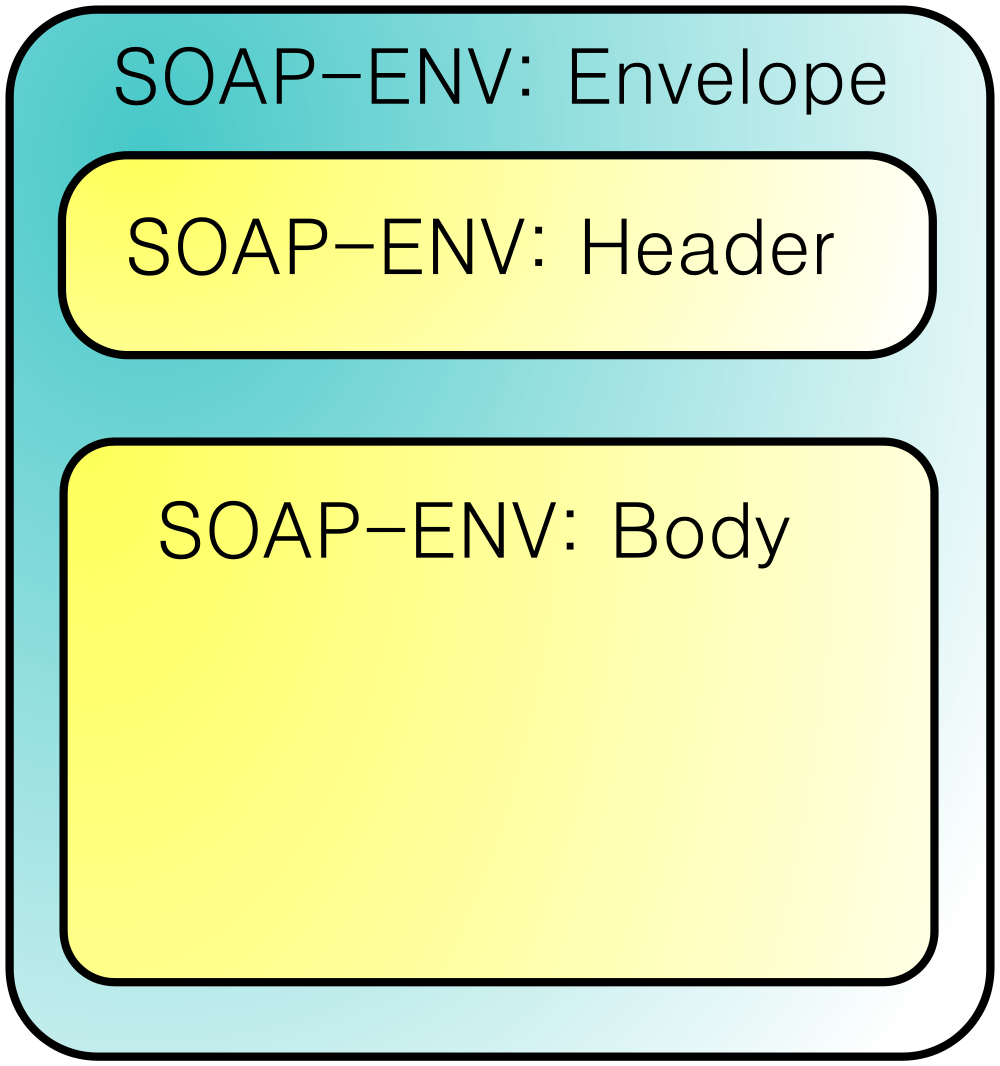
\includegraphics[width=\textwidth,keepaspectratio=true]{soap-envelope.png}
      % soap-envelope.png: 1000x1066 pixel, 72dpi, 35.28x37.61 cm, bb=0 0 1000 1066
  \end{columns}
\end{frame}

\begin{frame}
  \frametitle{Vzory pro výměnu zpráv}
  \framesubtitle{...neboli Message Exchange Patterns}

  \begin{block}{SOAP definuje tyto vzory výměny zpráv:}
    \begin{itemize}
      \item \highlighton{In-Only} \uv{void method(Object arg)}
      \item \highlighton{Robust In-Only} \uv{void method(...) throws Exception}
      \item \highlighton{In-Out} \uv{Object method(...) throws Exception}
      \item \highlighton{In Optional-Out}
      \vspace{4mm}
      \item Out-Only; Out-In: existují v rozšíření, nad \highlighton{HTTP nemožné}
    \end{itemize}
  \end{block}

  {\small Nezapomenout: typické chování výjimek v knihovnách}
\end{frame}

\begin{frame}
  \frametitle{Ukázka SOAP zprávy}
  
  \begin{example}
    SOAP zprávu si ukážeme naživo v praktické části
  \end{example}
\end{frame}

\section{WSDL}

\begin{frame}
  \frametitle{Něco málo o WSDL}

  \uv{Web Services Description Language}

  \begin{block}{WSDL}
    \begin{itemize}
      \item abstraktní jazyk pro popis rozhraní dané webové služby
      \item založený na \highlighton{XML} (xmlns, xmlschema, q-names)
      \item nezávislý na platformě i na jazyku implementace
      \item postačující pro kompletní implementaci klienta
      \item strojově zpracovatelný
      \begin{itemize}
        \item $=> \exists$ spousta generátorů různých kvalit
      \end{itemize}
    \end{itemize}
  \end{block}
\end{frame}

\begin{frame}
  \frametitle{Historie WSDL}
  \framesubtitle{...trocha dějinných souvislostí nikoho nezabije}  

  \begin{block}{WSDL historie:}
    \begin{itemize}
      \item 2000: WSDL 1.0 (Microsoft, IBM, Ariba)
      \item 2001: WSDL 1.1 pouze formalizace verze 1.0
      \begin{itemize}
        \item dodnes rozšířené (některé frameworky neumí 2.0)
      \end{itemize}
      \item 2003: WSDL 1.2 stále pouze \uv{working draft}
      \item 2008: WSDL 1.2 přejmenováno na 2.0
      \begin{itemize}
        \item získalo status W3C doporučení
        \item jednodušší, logičtější struktura (zpětně nekompatibilní)
        \item \highlighton{a proto si ukážeme tuto verzi}
      \end{itemize}
    \end{itemize}
  \end{block}
\end{frame}

\begin{frame}
  \frametitle{Struktura WSDL}
  \framesubtitle{...abychom se zorientovali}

  \begin{center}
    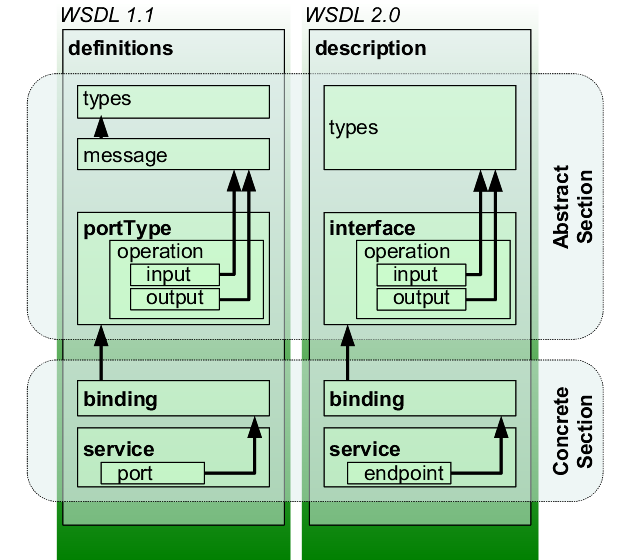
\includegraphics[height=.9\textheight,keepaspectratio=true]{wsdl-11-20.png}
    % wsdl-11-20.png: 632x560 pixel, 150dpi, 10.70x9.48 cm, bb=0 0 303 269
  \end{center}
\end{frame}

\begin{frame}
  \frametitle{Ukázka WSDL}

  \begin{example}
    Matěji, teď ukaž WSDL 2.0, které máš připravené
  \end{example}
\end{frame}

\section{Implementování}

\begin{frame}
  \frametitle{Přístupy k implementaci klienta}
  \framesubtitle{...jak nezešílet}

  \begin{alertblock}{Rozumná cesta}
    Každý rozumný programátor si základ vygeneruje z WSDL!
    \begin{itemize}
      \item nejlépe, když pak implementaci píše do jiných souborů
    \end{itemize}
  \end{alertblock}
\end{frame}

\begin{frame}
  \frametitle{Generovaní klienta z WSDL}
  \framesubtitle{...bylo by nudné to psát ručně}

	\begin{block}{Některé knihovny pro generování}
		\begin{itemize}
			\item \highlighton{Java:} Apache Axis, WSDL2Java, Spring
			\item \highlighton{Cocoa:} WSMakeStubs (zastaralé, bez úpravy kódu nefunkční)
		\end{itemize}    	
  \end{block}
	\begin{example}
		Matěji, a teď ukaž, jak se generuje javový kód. Pak nám tu ukaž funkčního klienta.
	\end{example}
\end{frame}

\begin{frame}
  \frametitle{Dynamicky vytvořený klient v Pythonu}
  \framesubtitle{...někdo generování nepotřebuje}

  \begin{example}
    Matěji, a teď ukaž, jak to lze celé udělat na 3 řádky.
    \begin{itemize}
      \item použita pythonová knihovna \highlighton{pysimplesoap}
    \end{itemize}
  \end{example}
\end{frame}

\begin{frame}
  \frametitle{Přístupy k implementaci serveru}
  \framesubtitle{Na co si dát pozor}

  \begin{block}{Jak implementovat}
    \begin{enumerate}
      \item Napsat WSDL, vygenerovat prázdnou implementaci
      \begin{itemize}
        \alert{\item pozor na pozdější úpravy}
      \end{itemize}
      \vspace{4mm}

      \item Naimplementovat server, vygenerovat WSDL
      \begin{itemize}
        \item typicky anotace k označení exportovaných metod
      \end{itemize}
      \vspace{4mm}

      \item Napsat obojí ručně
      \begin{itemize}
        \item \alert{nelze doporučit}, pouze pro otrlé
      \end{itemize}
    \end{enumerate}
  \end{block}
\end{frame}

\begin{frame}
  \frametitle{Server}
  \framesubtitle{...čím línější programátor, tým vyšší jazyk}

  \begin{block}{Frameworky pro psaní serverů}
    \begin{itemize}
      \item Apache Axis, Axis2 (Java/C/C++)
      \item .NET má podporu v základu
      \item Java Web Services
    \end{itemize}
  \end{block}

  \begin{example}
    Matěji, a teď ukaž, jak udělat server v Pythonu.
    \begin{itemize}
      \item znovu \highlighton{pysimplesoap} použitý ve frameworku \highlighton{web2py}
    \end{itemize}
  \end{example}
\end{frame}

\begin{frame}
  \frametitle{SOAP zpráva}
  \framesubtitle{...pohled pod pokličku}

  \begin{example}
    Matěji, teď se kouknem na SOAP zprávu zachycenou nebo někde zobrazenou
  \end{example}
\end{frame}

\begin{frame}
  \frametitle{Shrnutí}
  \framesubtitle{...co bych si tak měl zapamatovat}

  \begin{itemize}
    \item Web Services
    \begin{itemize}
      \item \highlighton{Malé} (REST) vs. \highlighton{Velké} (WSDL, SOAP)
    \end{itemize}

    \item REST
    \begin{itemize}
      \item \highlighton{http://abc.cz/data/42} + metody GET, PUT, DELETE
    \end{itemize}

    \item WSDL
    \begin{itemize}
      \item abstraktní strojově zpracovatelný XML \highlighton{popis web služby}
    \end{itemize}

    \item SOAP
    \begin{itemize}
      \item protokol upravující \highlighton{formát zpráv} a chování \highlighton{protějšků}
    \end{itemize}

    \item Implementování
    \begin{itemize}
      \item rozumnou část vygenerovat, \alert{pozor na udržovatelnost}
    \end{itemize}
  \end{itemize}
\end{frame}

\begin{frame}
  \frametitle{Zdroje}
  \framesubtitle{Pokud se chcete dovědět víc}
  \begin{thebibliography}{10}

  \beamertemplatearticlebibitems

  \bibitem{projekt-na-githubu}
    Zdrojáky serveru, klientů a prezentace
    \newblock {\tt http://github.com/strohel/web-service-test}

  \bibitem{wsdl}
    Předmluva k WSDL 2.0 specifikaci
    \newblock {\tt http://www.w3.org/TR/wsdl20-primer/}

  \bibitem{soap}
    Předmluva k SOAP 1.2 specifikaci
    \newblock {\tt http://www.w3.org/TR/soap12-part0/}

  \bibitem{xml-schema}
    XML Schema
    \newblock {\tt http://www.w3.org/TR/xmlschema-0/}

  \end{thebibliography}
\end{frame}

\begin{frame}
  \vspace{2cm}
  {\huge Otázky?}

  \vspace{3cm}
  \begin{flushright}
    Matěj Laitl, Matěj Novotný

    \structure{\footnotesize{matej@laitl.cz, mates.novotny@gmail.com}}
  \end{flushright}
\end{frame}

\end{document}
